\chapter{CONCLUSÃO}
\label{cap:conclusao}

Toda minha experiencia no Laboratório foi excepcional, obtive grande desenvolvimento profissional e pessoal, tendo que lidar com diversos problemas e pessoas.
Quando iniciei o estagio, meu conhecimento era somente relacionado ao que me foi ensinado na universidade ate o quinto período, oque na sua grande maioria eram conhecimentos sobre otimizações e códigos baixo nível.
Após alguns meses como estagiário, já possuía propriedade intelectual para opinar em decisões estruturais de projetos, tecnologias e ate mesmo dar prazos, logico que Após vários erros e muito estudo.
 
Os profissionais que tive o prazer de trabalhar sempre foram muito agradáveis e sempre agregaram muito no meu desenvolvimento.

No fim do meu estágio, posso dizer que já possuía propriedade para opinar em decisões importantes da empresa, como quais deviam ser as tecnologias principais e bibliotecas utilizadas.

Graças aos problemas resolvidos e projetos desenvolvidos no LEMAF, fui capaz de desenvolver minhas habilidades como desenvolvedor web e criar grande portfólio, abrindo diversas portas para o mercado de trabalho.
O estagio também me fez ter uma visão de todos os cargos e caminhos que poderia trilhar dentro da minha área de estudo, fazendo com que eu decidisse que realmente tinha como desejo e vocação ser desenvolvedor.

Meu atual emprego na empresa Equals só me foi oferecido por conta do conhecimento obtido em ReactJS e Spring. 

Posso dizer que os principais motivos de minha contratação foram minhas experiencias com as tecnologias e principalmente o desenvolvimento do Cria Design.

\begin{figure}[H]
\centering
\caption{Bilhete recebido da confraternização no fim de 2018} %legenda
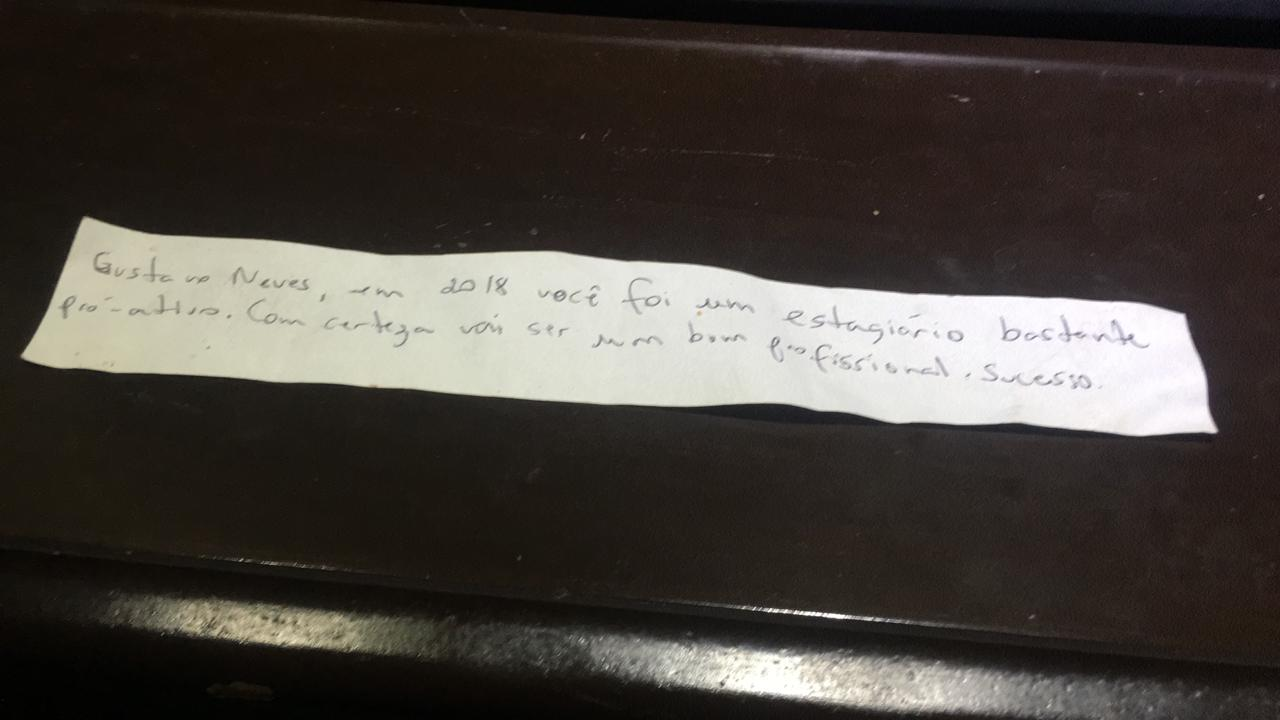
\includegraphics[scale=0.3]{agradecimento}\\  % o 0.9 indica 90% do tamanho original
% pdfLaTeX aceita figuras no formato PNG, JPG ou PDF
% figuras vetoriais podem ser exportadas para eps e depois convertidas para pdf usando epstopdf
\label{fig:exemplo} %rotulo para refencia
\end{figure}